{
% Image scale
\def\imgscale{0.34}

\textsf{Vi vil i det følgende forklare vores tanker bag en meget simpelt
fremgangsmåde, som har til formål at afgøre, om et billede opfylder det
gyldne snit. For at afgøre dette trækker vi regioner ud af billeder og
vurderer dem efter deres placering, størrelse og form. Afsnit
\ref{section_udtraek} vil forklare, hvordan selve udtrækningen af
regioner foregår, men her antager vi, at vi allerede har trukket
regionerne ud. I det følgende vil vi se på, hvornår en region ligger i
det gyldne snit, samt hvornår vi har med en interessant region at gøre.
}

\subsection{Regionens placering}
Når vi har trukket regioner ud af et billede og vil afgøre, om de ligger
i det gyldne snit, er det indlysende, at deres placering har en afgørende
betydning.  Vi vil nu komme frem til en definition, hvorved man kan
afgøre, om en region i billedet er placeret i det gyldne snit.

Vi starter med at se på et meget simpelt tilfælde, hvor en region ligger
placeret i det gyldne snit, som i figur \ref{pos_naiv_1}, hvor regionen,
vi betragter, er farvet sort.  Det gyldne snit markeres af en rød linje
--- et farveskema, der vil være gennemgående i det følgende --- og det
ses, at regionen nærmest tangerer linjen.

\begin{figure}[h]
    \begin{center}
        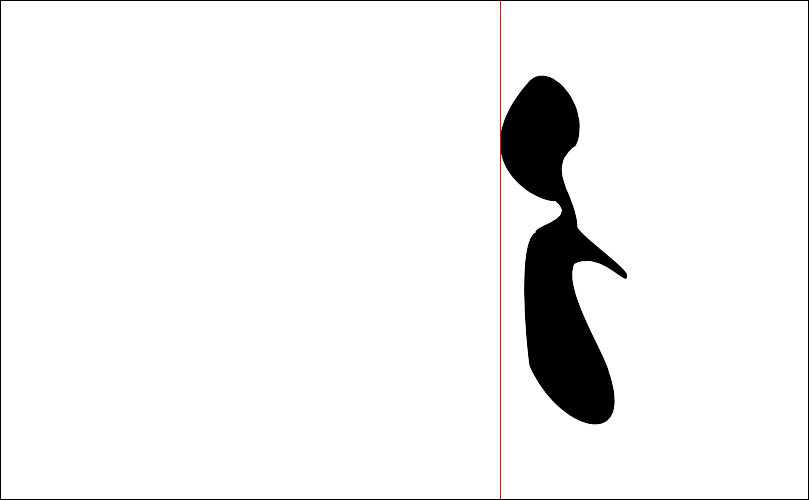
\includegraphics[scale=\imgscale,angle=0]{afsnit/vores_implementation/billeder/naiv_algoritme/naiv_positiv_blob_1}
    \end{center}
    \caption[En positiv region]{En region som tangerer det gyldne snit.
    Denne region er positiv.}
    \label{pos_naiv_1}
\end{figure}

%På grund af den måde, vi trækker regioner ud af billedet på,
%kan vi ikke være sikre på at regionen er fyldt helt ud til dens kanter,
%fordi der i disse områder stadig er stor overgang i farverne.  Dette
%bevirker at en regioner kan blive repræsenteret som mindre end de
%virkelig er.
I praksis er det dog sjældent tilfældet, at regioner ligger helt præcist
på snittet. Vi har i afsnit \ref{section_opdeling} defineret et margin,
som tager højde for dette. Hvis en region ligger inden for margin,
accepterer vi denne som liggende i snittet.
\begin{definition}
    Et \textbf{margin} er en udvidelse af vores snit, hvori vi vil
    godtage regioner, som liggende i snittet.
    \label{def_margin}
\end{definition}
I praksis betyder det, at vi \emph{ikke kun} betragter den linje, der
deler billedet ved det gyldne snit, men faktisk tager et bånd, sammensat
af en række snit, og bruger dette som et bredere gyldent snit.  Derved
behøver en region ikke at tangere det gyldne snit helt nøjagtig, for at
ligge i snittet, f. eks, er regionen i figur \ref{pos_naiv_margin_1}
placeret i det gyldne snit.  Vær opmærksom på, at vores margin, i de
følgende illustrationer, kan være stærkt overdrevet rent visuelt.
\begin{figure}[hb]
    \centering
    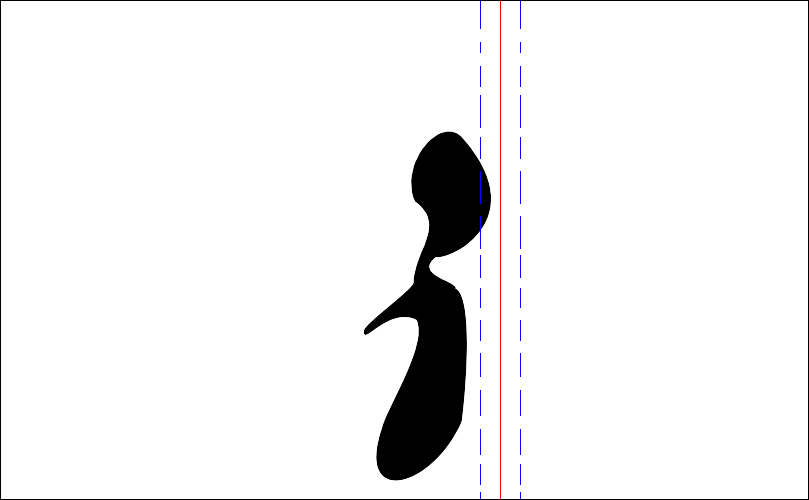
\includegraphics[scale=\imgscale,angle=0]{afsnit/vores_implementation/billeder/naiv_algoritme/naiv_positiv_blob_margin_1}
    \caption[Positiv region i margen]{En region, som ligger inden for
    den givne margin af det gyldne snit, betragtes som positiv. De blå
    stiplede linjer angiver vores margin.}
    \label{pos_naiv_margin_1}
\end{figure}

Til at afgøre, hvorvidt en region ligger inden for margin, har vi brug
for følgende definitioner:
\begin{definition}
    En regions \textbf{begrænsende rektangel}, er det mindste rektangel,
    der kan tegnes rundt om regionen, således at alle regionens
    ekstremer rører en side af dette rektangel. Eksempler, på
    begrænsende rektangler, ses i figur \ref{bbox_section}.
    \label{def_begraensende}
\end{definition}
\begin{definition}
    En side, af en regions begrænsende rektangel, kaldes for en regions
    \textbf{kant}.
    \label{def_region_kant}
\end{definition}
Ved at studere figur \ref{bbox_section} kan det ses, at en region skal
have mindst én kant inden for båndet om det gyldne snit, før vi kan
sige, at den ligger i snittet.
\begin{definition}
    Hvis en region har mindst én kant indenfor margin om det gyldne
    snit, så ligger denne region i det gyldne snit.
    \label{def_naiv}
\end{definition}

\begin{figure}[p]
    \begin{center}
        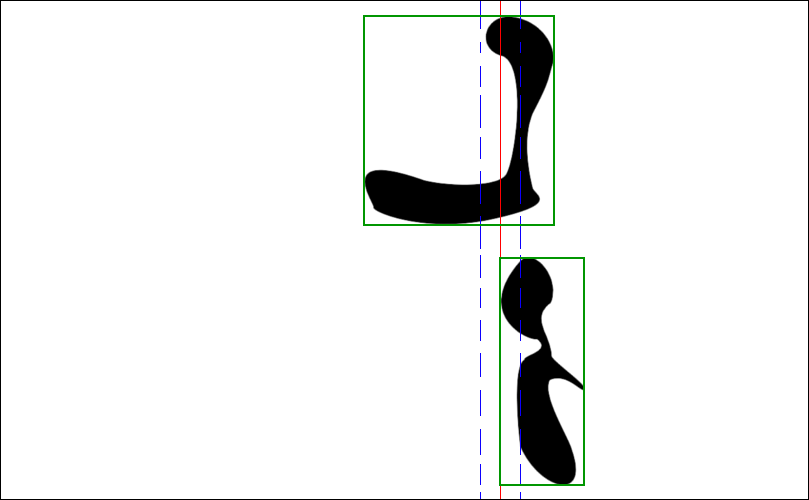
\includegraphics[scale=\imgscale,angle=0]{afsnit/vores_implementation/billeder/naiv_algoritme/bbox_section}
    \end{center}
    \caption[Begrænsende rektangler]{Den øverste region ligger ikke i
    det gyldne snit, da den ikke har nogen kanter inden for margin. Den
    nederste region, derimod, har én kant inden for margin og ligger
    derfor i det gyldne snit.} \label{bbox_section}
\end{figure}

\begin{figure}[p]
    \begin{center}
        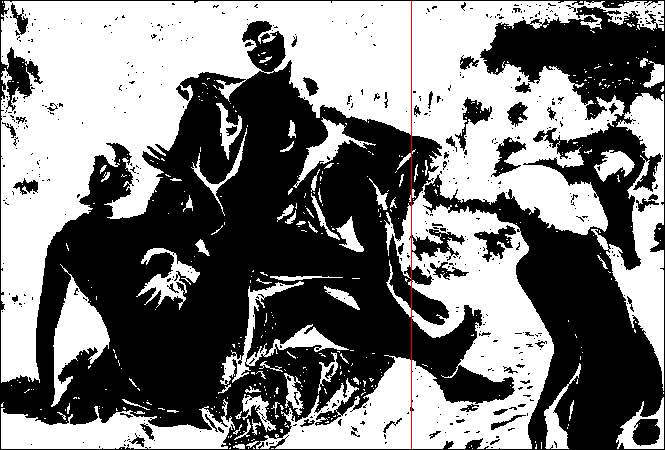
\includegraphics[scale=0.42,angle=0]{afsnit/vores_implementation/billeder/naiv_algoritme/bathers_mockup_blob}
    \end{center}
    \caption[Interessante regioner i praksis]{I praksis vil de
    fundne regioner være langt mere komplekse.}
    \label{realworld_example}
\end{figure}

Med ovenstående definition i tankerne kigger vi nu på, hvordan et
rigtigt billede kan tage sig ud, når vi vil finde regioner. I figur
\ref{realworld_example} ser vi, at der i dette tilfælde vil blive
udvalgt mange små regioner, som egentlig ikke kan tillægges nogen
betydning. Vi har derfor brug for at sortere uinteressante regioner fra.

\subsection{Interessante regioner}
Vi vil nu gå videre og opsætte nogle kriterier for, hvornår en region er
interessant.

\subsubsection{Regionens størrelse}
Når vi skal til at afgøre, hvorvidt en region er interessant, ser vi på
størrelsen af regionen.  Vi siger derfor, at en region skal have en vis
størrelse, før den kan betragtes som værende interessant. I praksis vil
regionens areal afspejle dens størrelse, hvor arealet er det antal
pixels, regionen optager i billedet.  Grænsen for et acceptabelt areal
skal sættes i forhold til billedets størrelse.

Omvendt er vi heller ikke interesserede i at få for store regioner med i
betragtningerne.  F.eks. vil en himmel i et maleri udgøre en ret stor
sammenhængende region.  De fleste af sådanne regioner vil dog ikke blive
taget i betragtning, fordi de krydser snittet.  Hvis vi kigger på det
meget simple billede i figur \ref{pos_naiv_1}, skal man også huske på, at
der faktisk vises to regioner. Den sorte skikkelse er en region, ligesom
den hvide baggrund er en region.  Baggrunden kan ikke siges at være en
interessant region, hvorfor det er vigtigt at sortere disse regioner
fra.

Hvor vi indtil videre kun har kigget på vertikale snit, vender vi nu
opmærksomheden mod et horisontalt.  Det generelle tilfælde vil være,
at en region kun er interessant i forhold til enten et vertikalt eller
et horisontalt snit.  Et eksempel på dette ses i figur
\ref{pos_horiz_naiv_margin_1}.

\begin{figure}[H]
    \begin{center}
        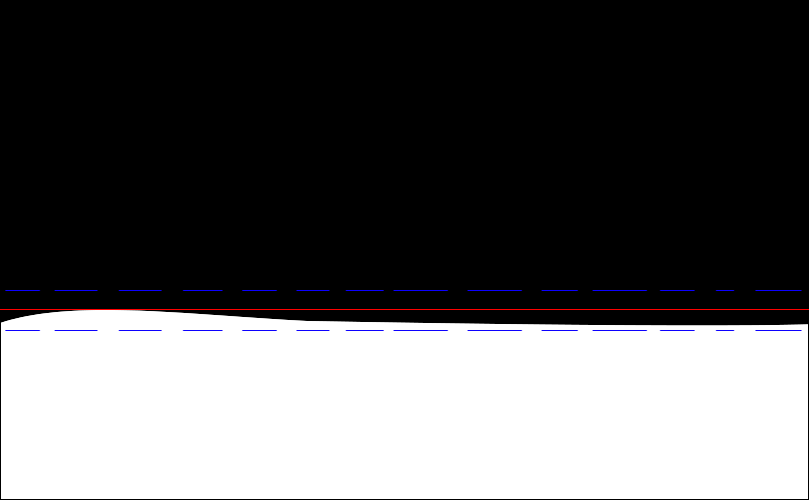
\includegraphics[scale=\imgscale,angle=0]{afsnit/vores_implementation/billeder/naiv_algoritme/naiv_horiz_positiv_blob_1}
    \end{center}
    \caption[Positiv horisontal region]{En positiv region med en
    kant i et horisontalt bånd.}
    \label{pos_horiz_naiv_margin_1}
\end{figure}
Det ses, at regionen i figur \ref{pos_horiz_naiv_margin_1} ikke
kan tages i betragtning i forhold til et vertikalt snit, da regionen,
uanset snittets placering, vil krydse dette.  Dog har regionen en kant
inden for et horisontalt bånd, og derfor kan den klassificeres som en
region, der ligger i det gyldne snit --- dog i forhold til et
horisontalt bånd.

\subsubsection{Regionens form}
Regionens form kan også give informationer om, hvorvidt vi har med en
interessant region at gøre.  I praksis er det dog meget svært at sige
noget om en regions fysiske form, men vi kan sige noget om dens masse.
En regions masse skal forstås, som forholdet mellem regionens areal og
arealet af regionens begrænsende rektangel.  Dette forhold giver
information om, hvor massiv en region er.  En massiv region vil være
mere interessant end en meget spinkel region.  Figur \ref{region_mass}
illustrerer to forskellige regioner med forskellig masse.
\begin{figure}[h]
    \begin{center}
        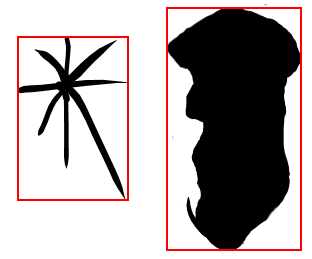
\includegraphics[scale=\imgscale,angle=0]{afsnit/vores_implementation/billeder/naiv_algoritme/bbox_area_ratio}
    \end{center}
    \caption[Regioners masse]{To forskellige regioner med vidt forskellige forhold
    mellem selve regionens areal og arealet af det rektangel, der
    begrænser regionen.}
    \label{region_mass}
\end{figure}
I praksis vil der blive fastsat en tærskelværdi, i forhold til et
billedes størrelse, for, hvor massiv en region skal være for at kunne
karakteriseres som interessant.

\subsubsection{Vurdering af interessante regioner}
Vi samler nu op på de ovenstående krav for bestemmelse af, hvornår en
region er interessant.

\begin{definition}
    For at en region kan betegnes som \textbf{interessant}, skal den
    \begin{enumerate}\label{naiv_regler}
            \renewcommand{\labelenumi}{(\alph{enumi})}
        \item have et areal større end en tærskelværdi, der sættes i
            forhold til billedets størrelse
        \item have en masse større end en tærskelværdi, der ligeledes,
            sættes i forhold til billedets størrelse,
    \end{enumerate}
    \label{def_interessant}
\end{definition}
I kapitel \ref{chap_afproevning} vil vi komme nærmere ind på, hvad
tærskelværdierne i praksis skal sættes til.

\subsection{Regioner liggende i det gyldne snit}
Vi har nu, at før at en interessant region ligger i det gyldne snit,
skal den opfylde definition \ref{def_naiv} og definition
\ref{def_interessant}.

Bemærk, at kun interessante regioner vil blive taget i betragtning, når
vi vil afgøre, om der ligger regioner i det gyldne snit. Dette betyder
også, at en region godt kan blive klassificeret som interessant uden
nødvendigvis at ligge i det gyldne snit og vice versa.

Bemærk, at selvom ovenstående fremgangsmåde tager udgangspunkt i det
gyldne snit, så kan metoden anvendes på ethvert snit i billedet ---
f.eks. kan vi bruge fremgangsmåden til at undersøge, om regioner i et
billede ligger i snittet ved en tredjedel.

\subsection{Begrænsninger}
Den naive tilgang har nogle begrænsninger, hvor den mest åbenlyse er, at
interessante regioner med symmetriakse i det gyldne snit, men med kanter
uden for margin, ikke ligger i det gyldne snit.  Regioner, hvor et
segment af denne faktisk ligger i båndet --- som den øverste region i
figur \ref{bbox_section} --- hvor den vertikale del faktisk ligger i
snittet, vil ikke blive udvalgt.  Det kræver en videre segmentering af
de fundne regioner, før en sådan region vil blive udvalgt.

Hvis vi betragter arbitrære snit i billedet, skal man være opmærksom på,
at en interessant region altid vil være positiv i fire snit; to i det
vertikale plan og to i det horisontale plan. Derfor, skal man, hvis man
ønsker at sammenligne positive regioner fra to arbitrære snit, sikre
sig, at deres margin ikke overlapper, da vi i dette tilfælde kan have
duplikater af de positive regioner.

}

% vim: set tw=72 spell spelllang=da:
